%!TEX root = ../DevaramaniS-[RnD-MT]Report.tex
\chapter{Dynamic equation of motion}\label{chap:dynamic}
The general dynamic equation of motion of a rigid body is expressed as \cite{featherstone2014rigid} \cite{shakhimardanov2015composable}, 
\begin{equation}
	\label{eq:dynamic}
	M(q)\ddot{q} + C(q, \dot{q}) = \tau 
\end{equation}

where, $M(q)$ represents mapping from motion domain($M^n$) to force domain($F^n$). $C(q, \dot{q})$ is the Coriolis and Centrifugal forces acting on the rigid body. Both these quantities are dependent on $q$, $\dot{q}$, $\ddot{q}$ and the physical model of rigid body \cite{featherstone2014rigid}

The dynamics problem is divided into forward and inverse dynamics. Computing the acceleration($\ddot{q}$), given the input forces($\tau$) is termed as \textit{forward dynamics} problem. Conversely, \textit{Inverse dynamics} problem calculates the forces, $\tau$ given accelerations $\ddot{q}$.

The rigid body is generally subjected to various motion constraints that changes the form of the dynamics equation. The extended equation is given by \cite{shakhimardanov2015composable},

\begin{equation}
\label{eq:extendeddynamic}
M(q)\ddot{q} = \tau_a(q) - \tau_c(q) -  C(q, \dot{q})
\end{equation}

In the above equation, $\tau_a$ represents input forces and $\tau_c$ is the constraint forces from the task specification.


\chapter{Pl{\"u}cker Notations for Spatial cross products}\label{chap:cross}

There are two spatial cross product operators expressed using Pl{\"u}cker notations are, $\times$ and $\times^*$ \cite{featherstone2014rigid}. The operators can be regarded as dual to each other. The matrix representation of these operators are deduced as \cite{featherstone2014rigid},

	\begin{equation}
	\label{eq:cross1}
		\hat v_O \times = \begin{bmatrix}
			\omega \\ v_O
		\end{bmatrix} \times = \begin{bmatrix}
			\omega \times & 0 \\
			v_O \times & \omega \times
		\end{bmatrix}
	\end{equation}
	
	and,
	
	\begin{equation}
	\label{eq:cross2}
	\hat v_O \times^* = \begin{bmatrix}
	\omega \\ v_O
	\end{bmatrix} \times^* = \begin{bmatrix}
	\omega \times & v_O \times \\
	0 & \omega \times
	\end{bmatrix}
	\end{equation}
	
\chapter{Representation of coordinate transforms}\label{chap:coordinate}	

In this section, the notations used to represent coordinate transformation matrices on motion and force vectors is presented. This follows the convention given in \cite{featherstone2014rigid}.

\begin{itemize}
	\item $\prescript{i+1}{}{X}_i$ - denotes coordinate transform from $i$ to $i+1$ coordinates of a motion vector,
	\item $\prescript{i+1}{}{X}_i^*$ - denotes coordinate transform from $i$ to $i+1$ coordinates of a force vector.
\end{itemize}

These transforms are related by the following equation \cite{featherstone2014rigid},
$$ \prescript{i+1}{}{X}_i^* = \prescript{i+1}{}{X}_i^{-T}$$

%\chapter{Kinematic Tree} 
%\label{chap:Kinematci-tree}
%
%A Kinematic tree comprises of interlinked segments. The \hyperref[kdl]{KDL} library provides a kinematic tree representation. Here, a single segments (KDL::Segment) is described as following~\cite{kinematictreeKDL},
%
%\begin{figure}[h!]
%	\label{fig:segment}
%	\begin{center}
%		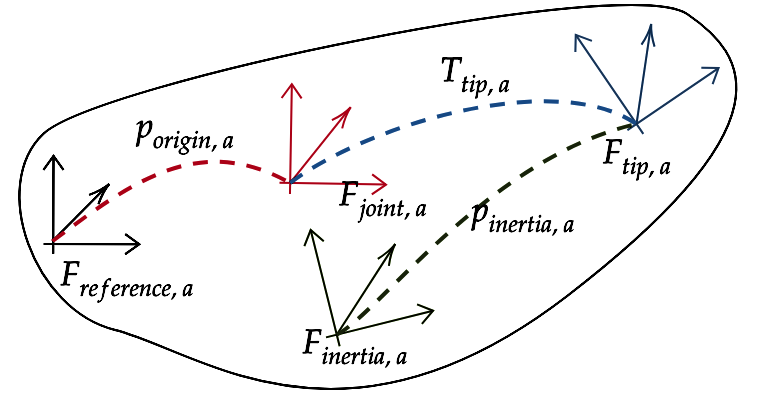
\includegraphics[scale=0.3]{images/segment}
%	\end{center}
%	\caption{KDL Segment}
%\end{figure} 
%
%The above figure represents a KDL segment composing of four frames,
%\begin{enumerate}
%	\item $F_{reference}$: A \textit{reference} frame (black colored frame) with respect to which other frames are expressed.
%	\item $F_{joint}$: A one DOF \textit{joint} frame (red) expressed about joint axis. The orientation of the frame is same as $F_{reference}$ and translation is given by $p_{origin, a}$.
%	\item $F_{inertia}$: A \textit{rotational inertia frame} (green) expressed with respect to \textit{tip frame} and $p_{inertia, a}$ is the translation vector. The frame is defined under KDL::RigidBodyInertia library.
%	\item $F_{tip}$: Frame attached at the tip of a segment. As seen in the figure \ref{fig:segment}, $F_{tip, a}$ is defined with respect to joint frame (blue) and transformation is given by $T_{tip, a}$ (by default: $T_{tip, a}$ is identity transformation). 
%\end{enumerate}
%
%A Kinematic tree is composition of branched KDL segments. An example is shown in the below figure (\ref{fig:kinematic-tree}) which describes a \textit{Kinematic tree} with two branches~\cite{kinematictreeKDL}. According to the convention, the joint frame of the succeeding segment is attached to tip frame of the preceding segment. Hence, the tip frames acts as the reference frame for the succeeding segments ($F_{tip, a} = F_{reference, b} = F_{reference, c}$). Similarly, the representation can be extended to multiple chains or interconnected segments.
%
%\begin{figure}[h!]
%	\label{fig:kinematic-tree}
%	\begin{center}
%		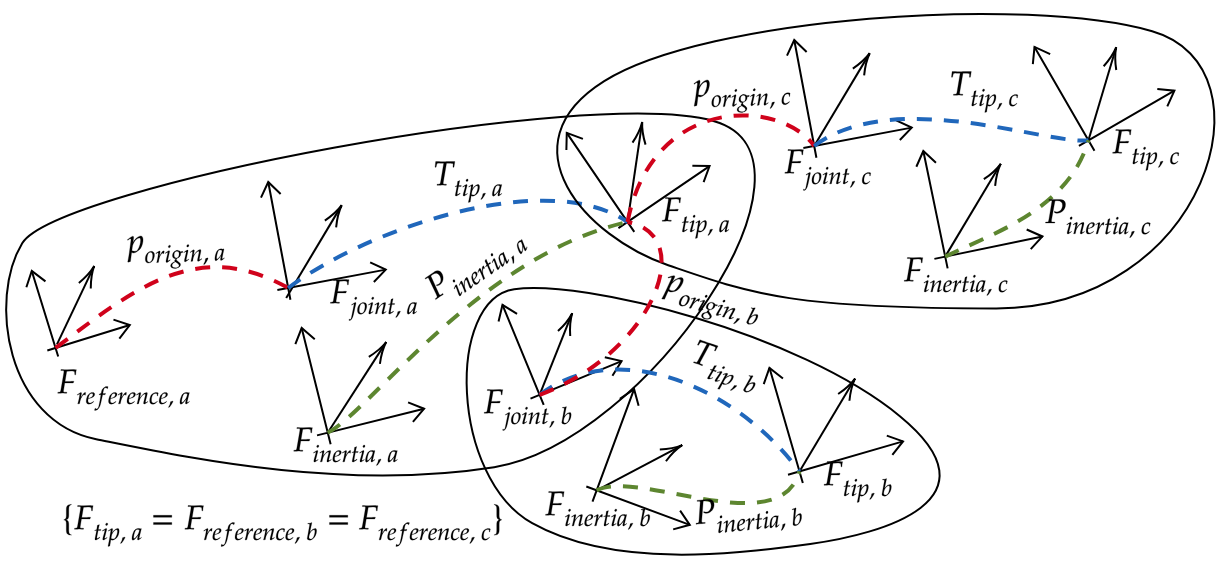
\includegraphics[scale=0.35]{images/kinematic-tree}
%	\end{center}
%	\caption{Kinematic tree representation in KDL}
%\end{figure}